\documentclass[
    paper=a4, 
    lang=en, 
    font=kpfonts, 
    hanging-titles=true,
    draft
]
{skrapport} 
\colortheme{skdoc}

% meta info
\title{
    {Information Theoretic Error Bounds on NISQ Learning Systems} \\
    {\large B.Tech Project I}
    }
\author[sgambhir@iitb.ac.in]{Sankalp Gambhir}
\date{\today}

% setup packages, macros, notes
\newcounter{notes}
\setcounter{notes}{1}
% general formatting and stuff
\usepackage{graphicx}
\usepackage{xcolor}
\usepackage{ragged2e}
\usepackage{ifthen}
\usepackage{lineno}
\usepackage{booktabs}
\usepackage{subcaption}

% subject specific
\usepackage{amsmath, amssymb, amsthm}
\usepackage{physics, physconst, physunits}
\newtheorem{axiom}{Axiom}

% drawing
\usepackage{pstricks}
\usepackage{tikz, tkz-orm, pgfplots}
\usetikzlibrary{arrows,shapes,backgrounds,decorations.markings}
\usetikzlibrary{matrix,positioning,decorations.pathreplacing,calc,tikzmark}
\pgfplotsset{width=7.5cm,compat=1.16}
\usepgfplotslibrary{fillbetween}

% links and citations
\usepackage{hyperref, bookmark}
\hypersetup{hidelinks} % hide boxes around links ew
\usepackage{csquotes}
\usepackage[
    style=numeric,
    sorting=none
]{biblatex}
\addbibresource{biblio.bib}

% notes
\newcommand{\notes}[1]{}

\ifthenelse{\value{notes} > 0}{
    \renewcommand{\notes}[1]{{\textcolor{red}{[Note: #1]}}}
}{}

% actual macros
\newcommand{\reals}{\ensuremath{\mathbb{R}}}
\newcommand{\naturals}{\ensuremath{\mathbb{N}}}
\newcommand{\complex}{\ensuremath{\mathbb{C}}}
\newcommand{\featurespace}{X}
\newcommand{\labelset}{L}


\begin{document}

    \begin{titlepage}
        \maketitle
        \begin{abstract}
            Bla bla.
        \end{abstract}        
    \end{titlepage}

    \tableofcontents

    \section{Introduction}
        \label{sec:intro}
        % intro.tex

% intro to problems of learning and classification
There has been long standing interest in learning from data and extrapolating
experimental data to make useful predictions using computers about as long as
computers have existed. In the last few decades, with computing power
skyrocketing exponentially coupled with leaping advances in theory of learning
systems and statistical inference, these problems became tractable and
eventually came into use ubiquitously. With applications ranging from facial
detection systems for surveillence to identifying cosmic objects for cosmology,
they have found widespread adoption in industry and academia. With their advent,
however, has come an ever rising need for computing power. This has found data
centers of unprecendented scales consuming enormous amounts of power to provide
the instant predictions we've come to rely on.

% intro to how quantum may solve it
With snowballing energy and space requirements of classical computers in the
form of GPU clusters and ASICs, there has been a spark of interest in offloading
this computation onto quantum computers, which, till recently, have largely
remained a rare species spotted only in labs surrounded by helium-cooled
superconductors and white-coated predators. Current scales of available quantum
computers, however, still lack the power required to fully tackle these
challenges while maintaining reliable error-levels or adding their own error
checking and correction. This has motivated using quantum computers to run
bottnecked computational subroutines with classical control systems. These
systems generally lack error correction, and thus earn themselves the title of
`noisy'. These form the basis of computation considered in this thesis, Noisy
Intermediate-Scale Quantum (NISQ) computers.

Connecting a quantum computer to a classical puppeteer is not expected to come
without its own issues either. It constrains the architecture and is itself
bottlenecked on both ends, first by the parameter transfer and configuration
from the classical to the quantum, then finally by the detectors on the quantum
side to the classical. In this thesis, we focus on the former, discussing the
limits of computation and computational precision achievable with this hybrid
architecture.

% report structure
\subsection{Structure}
In \autoref{sec:prelim}, definitions and relevant results in classical
computing, physics, and quantum information are presented. \notes{Extend this.}

\subsection{Outline of New Results}
\notes{Add summary of results at the end.}

    
    \section{Preliminaries}
        \label{sec:prelim}
        % prelim.tex

% classical prelims
\subsection{Classical Computing}
% learning
\subsubsection{Learning Problem}
Learning \cite{cristianini2000introduction} can be broadly defined as attempting
to learn the input-output pattern given sample data. For this thesis, we
consider three major categories of learning problems:

\begin{itemize}
    \item Binary Classification --- input points in a chosen domain, and a
    binary output label for each point.
    \item Multi-Label Classification --- input points in a chosen domain, and
    one of \(n\) labels as output for each point.
    \item Regression --- input points in a chosen domain with real-valued output.
\end{itemize}

% classification problem
\subsubsection{Classification Problem}
We take as input elements \(\{x_i\}\), generally called \emph{feature vectors},
in a chosen domain \(\featurespace\) called the \emph{feature space} and output
an element from a finite set \(\labelset = {l_i}\) of labels. \notes{Add a nice picture}

The problem is called binary classification if \(\absolutevalue{\labelset} =
2\).

Formally, we attempt to learn a function \(f: \featurespace \to \labelset\)
given a set of inputs in the domain, and possibly paired output labels.

The problem proceeds in two manners given the form of inputs: if provided
input-output pairs, the problem is called a \emph{supervised learning problem},
while attempting to learn a set of labels given just (clustered) inputs is
called \emph{unsupervised} learning. We focus on supervised classification here.

The set of input-output pairs provided is called the \emph{training data}.

Given the difficulty of working with discretized domains, the input domain is
generally converted to be a subset of a Euclidean space, using a suitable
\emph{embedding function}.

% embedding
\subsubsection{Embedding}
An embedding of \(X\) in \(Y\) is a function \(f:X \to Y\) that is injective and
structure-preserving. The exact restrictions on the map to be
structure-preserving depend on the structures of the domain and the codomain
\cite{sankappanavar1981course}. It is denoted here as \(f:X\hookrightarrow Y\).

For example, a topological embedding, i.e., the embedding of a topological
space, will be restricted to preserve its associated structure of open sets. A
field embedding, similarly, will be restricted to preserve the field operations
\(+\) and \(\times\).

For a given arbitrary feature space \(\featurespace\), it is generally embedded
into \(\reals^n\) for some \(n\).

% linear classification
\subsubsection{Linear Classification}
Classification generally proceeds by producing linear functions as candidate
(supplemented with a discretization function) labelling functions and fitting
them to the training data. For simplicity, we first restrict the discussion to
binary classifiers.

\begin{figure*}[h]
    \centering
    \begin{subfigure}{0.48\textwidth}
        % unsep bs
        \centering
        \begin{tikzpicture}[>=stealth']
            % Draw axes
            \draw [<->,thick] (0,5) node (yaxis) [above] {}
                  |- (5,0) node (xaxis) [right] {};
            % draw negative dots
            \fill[black] (0.5,1.5)    circle (3pt);
            \fill[black] (2.0,2.7)   circle (3pt);
            \fill[black] (1.0,3.4)   circle (3pt);
            \fill[black] (3.0,2.0)   circle (3pt);
            \fill[black] (1.5,1.0)   circle (3pt);
            \fill[black] (2.5,0.5)   circle (3pt);
            % draw positive dots
            \draw[black] (3.5,1.5)     circle (3pt);
            \draw[black] (2.5,1.7)     circle (3pt);
            \draw[black] (1.5,2.3)     circle (3pt);
            \draw[black] (0.5,3.0)     circle (3pt);
          \end{tikzpicture}
          \caption{Unseparated data}
    \end{subfigure}
    \begin{subfigure}{0.48\textwidth}
        % nice and separated
        \centering
        \begin{tikzpicture}[>=stealth']
            % Draw axes
            \draw [<->,thick] (0,5) node (yaxis) [above] {}
                  |- (5,0) node (xaxis) [right] {};
            % separator
            \draw (-0.5, 4.0) -- (4.0,0.0) [dashed];
            % draw negative dots
            \fill[black] (0.5,1.5)    circle (3pt);
            \fill[black] (1.5,1.7)    circle (3pt);
            \fill[black] (2.0,0.5)    circle (3pt);
            \fill[black] (1.0,2.3)    circle (3pt);
            \fill[black] (2.5,0.6)    circle (3pt);
            % draw positive dots
            \draw[black] (3.5,1.5)     circle (3pt);
            \draw[black] (2.5,2.0)     circle (3pt);
            \draw[black] (1.5,3.5)     circle (3pt);
            \draw[black] (1.0,4.0)     circle (3pt);
            \draw[black] (0.5,3.8)     circle (3pt);
          \end{tikzpicture}
          \caption{Strongly separated data}
    \end{subfigure}
    \caption{The magic of the (strong) separation axiom.}
\end{figure*}

Given a set of points which, due to an embedding, may be assumed to be in
\(\featurespace\subseteq\reals^n\), attempting to classify them may still be an
arduous task if the spatial regions corresponding to the labels are intertwined.
Thus, to make the problem tractable, we restrict the data to be \emph{strongly}
separated, i.e., any labelling function \(f:\featurespace \to \labelset\) that
agrees with the training data \notes{try to write separation properly}.

% probability distribution separation? TODO
% inner product space? TODO

% svm
\subsubsection{Support Vector Machine}
A support vector machine is a classifier model which constructs a hyperplane or
a set of hyperplanes in the feature space optimising classifier separation
depending on the objective \cite{cortes1995support}.

We will synonymously use the terms `Support Vector Machine' and that of its
common model `Maximal Margin Classifier', which is more appropriately what we
use here.

As the name suggests, a maximal margin classifier SVM tries not only to
construct a set of hyperplanes, but to find the set such that their margin from
the data is maximised. This builds upon the intuitive idea of a good separator
being further away from the given data points. See \autoref{fig:maxmargin}.


\begin{figure*}[h]
    \centering
    \begin{subfigure}{0.48\textwidth}
        % unsep bs
        \centering
        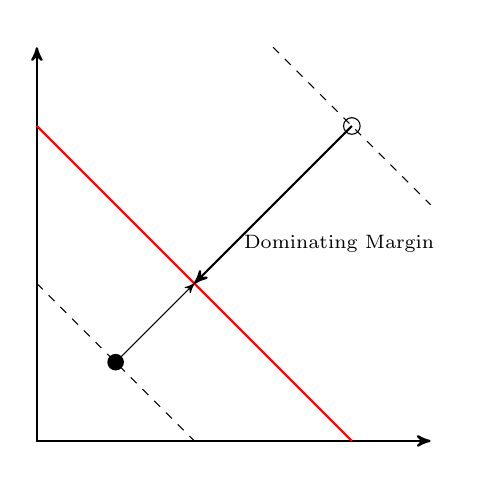
\begin{tikzpicture}[>=stealth']
            % Draw axes
            \draw [<->,thick] (0,5) node (yaxis) [above] {}
                  |- (5,0) node (xaxis) [right] {};
            % classifier
            \draw[red, thick] (0.0, 4.0) -- (4.0, 0.0);
            \draw[->, thin] (1.0, 1.0) -- (2.0, 2.0);
            \draw[->, thick] (4.0, 4.0) -- node[near end, right] {\scriptsize Dominating Margin} (2.0, 2.0);
            \draw (3.0, 5.0) -- (5.0, 3.0) [dashed];
            \draw (0.0, 2.0) -- (2.0, 0.0) [dashed];
            % draw negative dots
            \fill[black] (1,1)    circle (3pt);
            % draw positive dots
            \draw[black] (4,4)     circle (3pt);
          \end{tikzpicture}
          \caption{Unoptimized margins}
    \end{subfigure}
    \begin{subfigure}{0.48\textwidth}
        % nice and separated
        \centering
        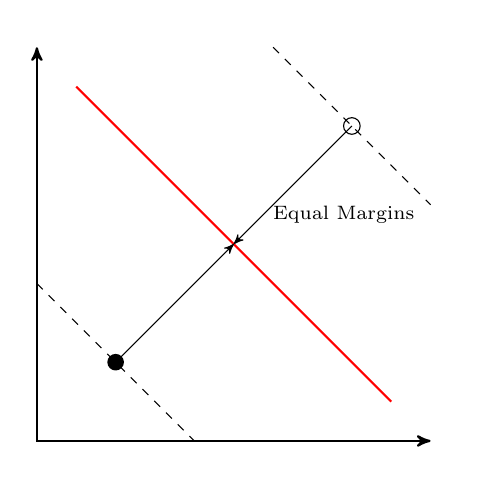
\begin{tikzpicture}[>=stealth']
            % Draw axes
            \draw [<->,thick] (0,5) node (yaxis) [above] {}
                  |- (5,0) node (xaxis) [right] {};
            % classifier
            \draw[red, thick] (0.5, 4.5) -- (4.5, 0.5);
            \draw[->] (1.0, 1.0) -- (2.5, 2.5);
            \draw[->] (4.0, 4.0) -- node[near end, right] {\scriptsize Equal Margins} (2.5, 2.5);
            \draw (3.0, 5.0) -- (5.0, 3.0) [dashed];
            \draw (0.0, 2.0) -- (2.0, 0.0) [dashed];
            % draw negative dots
            \fill[black] (1,1)    circle (3pt);
            % draw positive dots
            \draw[black] (4,4)     circle (3pt);
          \end{tikzpicture}
          \caption{Maximal margin classifier}
    \end{subfigure}
    \caption{Illustration of different margins for hyperplanes.}
    \label{fig:maxmargin}
\end{figure*}

Formally, we characterize a hyperplane in \(\reals^n\) as a pair \((\vecw, b)\),
with \(\vecw \in \reals^n\) and \(b \in \reals\), such that for all points
\(\vecx\) on the hyperplane

\begin{gather*}
    \innerprod{\vecw}{\vecx} + b = 0~.
\end{gather*}

Geometrically, \(\vecw\) is the vector normal to the hyperplane, and \(b\)
is the bias or offset from origin.

Note that by moving to \(\reals^{n+1}\), we can convert the hyperplane to one
without bias (passing through the origin)

\begin{gather*}
    \innerprod{\vecw}{\vecx} + b = 0~,\\
    \innerprod{(\vecw \oplus \begin{pmatrix}
        b
    \end{pmatrix})} {(\vecx \oplus \begin{pmatrix}
        1
    \end{pmatrix})} + 0 = 0~.
\end{gather*}

which is the hyperplane \((\vecw \oplus \begin{pmatrix}b\end{pmatrix}, 0)\) in
\(\reals^{n+1}\). So, without loss of generality, we work with hyperplanes
without bias.

Now, given the training dataset \({(\vec{x_i}, y_i)}\), with \(y_i = \pm 1\), we
can write constraints on \(\vecw\) as

\begin{gather}
    \forall i\; y_i \cdot \innerprod{\vecw}{\vec{x_i}} > 0~,
\end{gather}

that is, \(x_i\) is on the same side of the hyperplane as indicated by \(y_i\)
as the sign of the inner product corresponds to the same. 

By scaling \(\vecw\) (without changing the hyperplane), we can construct the
constraint system

\begin{gather}
    \forall i\; y_i \cdot \innerprod{\vecw}{\vec{x_i}} \geq 1~.
\end{gather}

Since we are scaling \(\vecw\), we choose an appropriate optimization target,
its norm.

Since this is a constrained optimization, we write its Lagrangian

\begin{gather}
    \mathcal{L}(\vecw, \vec{\alpha}) = \frac{1}{2} \innerprod{\vecw}{\vecw} + \sum_i \alpha_i \left[y_i \cdot \innerprod{\vecw}{\vec{x_i}}\right]~,
\end{gather}

where \(\{\alpha_i\}\) are the Lagrangian multipliers. For the optimal solution,
the Lagrangian is stationary, i.e.,

\begin{gather}
    \frac{\partial \mathcal{L}(\vecw, \vec{\alpha})}{\partial \vecw} = 0~,\nonumber\\
    \vecw - \sum_i \alpha_i y_i \vec{x_i} = 0~.
\end{gather}

Substituting this expression for \(\vecw\) in the Lagrangian itself, we get \notes{work out the substitution}

\begin{gather}
    \mathcal{L}(\vecw, \vec{\alpha}) = \frac{1}{2} \innerprod{\vecw}{\vecw} + \sum_i \alpha_i \left[y_i \cdot \innerprod{\vecw}{\vec{x_i}}\right]~,
\end{gather}

By maximising this Lagrangian with respect to the parameters \(\{\alpha_i\}\),
we obtain an optimal \(\vecw\) which is the maximum margin classifier.

With \(\vecw\) fixed at its optimal value, we get a simple computational method
to classify all new incoming points \(\vecx \in \reals^n\), given by

\begin{gather}
    \text{sgn}(\innerprod{\vecw}{\vecx})
\end{gather}

returning a label \(\pm 1\) (or anomalously zero, if you happen to pick a point
on the hyperplane, which can be remedied by making one side's boundary soft).

% how optimise
\subsubsection{Optimisation Techniques}
Gradient descent or st. \notes{expand}

% error introduction
\subsubsection{Generalisation Error}
Hello \notes{read about gen error and write here}

% qm prelims
\subsection{Quantum Regime}
\notes{add a general introduction}

% schrodinger
\subsubsection{Schr\"odinger Equation}

% hilbert space
\subsubsection{Hilbert Space}

% quantum computer
\subsubsection{Quantum Computation}

% quantum embedding
\subsubsection{State Construction and Embedding}

% measurement
\subsubsection{Measurement}

    \phantomsection
    \addcontentsline{toc}{section}{References}
    \printbibliography
\end{document}